% figures/fig3_grid.tex -- float wrapper for FIGURE 3, the matched six-cell grid.
%
% Image produced by figures/fig3_grid.py (PDF at figures/out/fig3_grid.pdf,
% audit record at figures/out/fig3_grid_data.json).  Drawn at final size
% (5.5in single column); include with width=\linewidth only, never \resizebox.
%
% PROVENANCE.  Every number in the image is recomputed at build time from
% runs/eval_ours/clean_p0_<CELL>_s<N>/boltz_independent_records.csv by the
% recipe "drop pert_id == 0, keep xtb_ok, per-parent Pearson r(log q_theta, -E/kT),
% mean over the 120 parents"; the launched/completed/diverged triples are a
% checkpoint census over runs/p0/p0_<CELL>_s<N>.  The generator refuses to draw
% unless all 24 per-seed values, all six cell means/sems, all six triples and
% all six contrasts reproduce the independently verified values.  The Welch t
% values stay inside that gate and inside the audit JSON; none is rendered.
%
% RULINGS SATISFIED.  (i) This float replaces the per-seed grid table in the
% main text: the numeric table is not the communication device, the seed points
% are.  (ii) The verified force cell is clean_p0_E_force_*, not E2; the post-hoc
% relaunches D_energy_s6/s7/s9 and F_both_s6..s10 are excluded, because no
% diverged seed is ever replaced.  (iii) The reference-included
% mean_pearson_r in boltz_independent.json is never read.  (iv) NO inferential
% statistic is rendered anywhere in this float.  Panel (b) is an EFFECT-SIZE
% panel: six differences of cell means with the propagated standard error of
% the difference as a descriptive whisker.  No Welch t, no p-value, and no
% "significant" / "n.s." label appears in the image or in the caption.
%
% C11 (this pass).  Panel (a)'s title now conditions on completion explicitly
% ("Among completed runs, ..."), and the caption no longer offers survivorship
% as an alternative reading of cell D.  The claim it makes instead is checkable:
% the three completed D seeds (0.452, 0.398, 0.412) lie above every control
% seed (A max 0.234, B max 0.243, C max 0.232), and the direction agrees with
% the corrected earlier checkpoint family, whose 93-parent primary endpoint is
% 0.369 (value) vs 0.200 (FM only) in figures/out/scale_primary.json
% -> dropref/{a3_energy,a1_fm_only}/per_seed/*/primary_93/pearson_r.  What the
% caption does NOT claim is an unconditional magnitude for D or F.
% C12 (figure-editor pass, reviewer item 8).  The PDF is placed at
% width=\linewidth again, as this header always specified, and the generator
% draws its canvas at exactly 5.50 x 2.35 in with an explicit (non-tight)
% bounding box.  Placed size therefore equals drawn size, every in-figure point
% size is a page point size, and nothing renders below 7 pt.  The canvas height
% is the height the float already occupied (3.05 in x 0.76 = 2.318 in), so the
% vertical footprint is unchanged; the enlargement comes entirely from the 24%
% of the column that the fractional placement used to waste as margin.  The
% in-panel line repeating "120 held-out parents / reference geometry dropped /
% independent GFN2-xTB evaluator" is deleted: the caption below states all three
% and the line was the least legible object on the page.
\begin{figure}[t]
\begin{center}
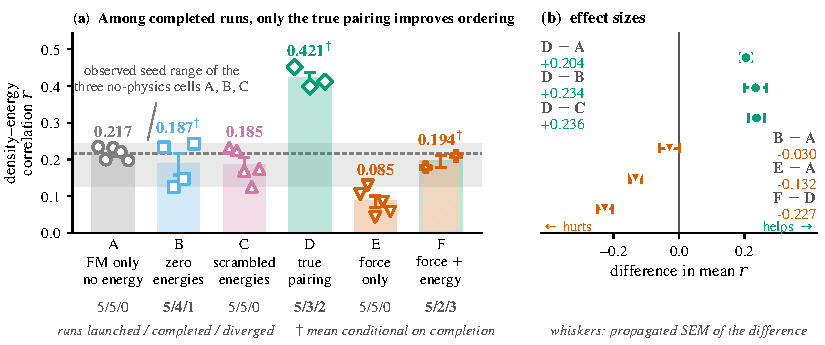
\includegraphics[width=\linewidth]{figures/out/fig3_grid.pdf}
\end{center}
\caption{Archived readout results; likelihood labels in the plots refer to $\widehat\ell_\theta$, not a validated generator density. \textbf{A matched six-cell grid isolates what the energy term
contributes.} Population: 120 held-out parents, reference geometry dropped, 8
displaced geometries each, scored by an independent GFN2-xTB evaluator, not the
eSEN training teacher. Metric: the per-parent density--energy correlation $r$,
per cell as the mean over completed training seeds (whisker: standard error
over seeds) with every completed seed drawn, and in (b) as effect sizes:
differences of cell means, whiskers the propagated descriptive SEM of the
difference rather than a confidence interval. Cells A--F are defined in
\Cref{sec:ablation}; runs launched / completed / diverged are printed under each
cell, because completion is objective-dependent. Only the true geometry--energy
pairing separates: every completed D seed lies above the shaded band, the
observed seed range of A, B and C; the zero-energy and scrambled cells do not,
and the gradient baseline falls below. \textbf{Cells B, D and F lost seeds to divergence}
($\dagger$), so their means are conditional on completion and the D and F
unconditional magnitudes are not identified. Panel detail in
\Cref{app:figdetail}.}
\label{fig:grid}
\end{figure}
